% Minimal preamble; kept only your content
\documentclass[pdflatex,sn-mathphys-ay]{sn-jnl}
\usepackage{graphicx}
\usepackage{amsmath,amssymb,amsfonts}
\usepackage{amsthm}
\usepackage{booktabs}
\usepackage{multirow}
\usepackage{xcolor}
\usepackage{algorithm}
\usepackage{algorithmicx}
\usepackage{algpseudocode}
\usepackage{listings}
\begin{document}
\title{From Tensors to Novelties: Low-Dimensional Representations for Anomaly Detection in Multispectral Imagery}

\author*[1]{\fnm{Anthony C.} \sur{Chan}}\email{anthonycchan@gmail.com}
\affil*[1]{\orgdiv{H. Milton Stewart School of Industrial \& Systems Engineering (OMSA- Practicum Summer 2024)}, \orgname{Georgia Institute of Technology}, \city{Atlanta}, \state{GA}, \country{USA}}

\keywords{tensor decomposition, CP, Tucker, anomaly detection, multispectral data}

\abstract{Anomaly detection in image datasets often benefits from reducing high-dimensional inputs into compact, interpretable representations. Tensor decomposition provides a principled way to achieve this by factorizing complex data into low-dimensional components that preserve both spatial and spectral structure. In this work, I investigate how tensor decomposition can be combined with standard anomaly detection models to identify novel patterns in image data. I evaluate two decomposition strategies - global CP (PARAFAC) and per-sample Tucker decompositions as feature extraction steps. The resulting low-dimensional coefficients are then used to train one-class classifiers, including one-class support vector machines (OC-SVMs), autoencoders (AE), and isolation forests (IF). Models are trained on typical examples only, identifying anomalies as observations poorly explained by the learned representation during training. To demonstrate the methodology, I apply it to multispectral images from the Mars Science Laboratory Curiosity rover, a dataset characterized by scarce labeled anomalies. The experiments reveal a trade-off: CP decomposition provides substantial improvements under locally coherent training conditions, while Tucker decomposition delivers more consistent gains under randomized sampling. These results highlight tensor decomposition as an effective methodology for coupling dimensionality reduction with anomaly detection, with CP suited to structured regimes and Tucker preferred in more heterogeneous settings, with potential applications in planetary exploration, medical imaging, and industrial inspection.}

\maketitle

\section{Introduction}
Tensor decomposition, such as PARAFAC/CP \citep{Harshman1970} and Tucker \citep{Tucker1966}, has been used successfully for exploratory multi-way factor analysis in psychometrics and social sciences and continues to be a central tool across disciplines \citep{KoldaBader2009}. Anomaly detection aims to identify patterns in data that have not been previously observed \citep{Markou2003a,Markou2003b,Chandola2009,Pimentel2014}. When combined, these methods can be used to identify novel features in low-dimensional images, such as those collected during rover-based planetary exploration missions. For example, \citep{Kerner2020} compared multiple anomaly detection techniques on multispectral images from the Mars Science Laboratory (MSL) Curiosity rover, demonstrating the importance of unsupervised approaches for prioritizing scientifically interesting observations under constraints of bandwidth and mission time.

Beyond planetary exploration, low-dimensional anomaly detection has been applied in diverse fields, such as the detection of lesions in magnetic resonance imaging \citep{Kim2021} and the identification of surface cracks in industrial quality-control settings \citep{Tabernik2019}. These examples highlight the versatility of combining dimensionality reduction with anomaly detection in domains where anomalies are rare, labels are scarce, and interpretability is critical.

The present study builds on \citet{Kerner2020} by exploring tensor decomposition as a feature extraction step for anomaly detection in rover-based multispectral images. A key challenge in this domain is the scarcity of labeled novel data, which reflects real-world operational conditions. To address this, I adopt a one-class learning framework: models are trained on typical (non-novel) examples, and novel observations are identified as those poorly explained by the learned representation \citep{Pimentel2014}. 

I compare multiple tensor decomposition strategies—global CP (PARAFAC) and per-tile Tucker decomposition—and use the resulting low-dimensional representations as inputs to established anomaly detection models, including one-class support vector machines (SVM), autoencoders, and isolation forests. Performance is evaluated in terms of ROC–AUC under two dataset configurations: an in-order split using the first 1,500 samples for training and a randomized selection drawn from the full dataset. The results show a trade-off between potential and robustness. CP decomposition provides substantial improvements over baselines when the training data is locally coherent, while Tucker decomposition yields more consistent performance across heterogeneous, randomized sampling. These findings demonstrate that tensor decomposition can meaningfully enhance anomaly detection pipelines, with CP suited to structured subsets and Tucker preferred for diverse data regimes.

\section{Related Work}
\subsection{Tensor decompositions}

\textbf{CP/PARAFAC/CANDECOMP.} \citet{Harshman1970} introduced the PARAFAC/CP model, which represents a tensor as a sum of rank-1 outer products with one loading vector per mode, enabling extraction of shared components across modes. 
\textbf{Tucker.} \citet{Tucker1966} proposed the Tucker model, which reduces a tensor to a smaller core coupled with one factor matrix per mode; in this study, the (vectorized) core serves as a compact representation of each training image. 
\textbf{Algorithms and surveys.} An efficient way to compute Tucker factors is via the Higher-Order Singular Value Decomposition (HOSVD), which computes per-mode left singular vectors to assemble orthonormal factor matrices and obtain a core tensor \citep{DeLathauwer2000a}. For comprehensive coverage of CP and Tucker notation, algorithms, uniqueness, constraints, and complexity, see \citet{KoldaBader2009}.

\subsection{Anomaly (novelty) detection methods}
\textbf{Surveys and motivation.} \citet{Chandola2009,Pimentel2014} review anomaly/novelty detection, including anomaly taxonomies, application constraints, and evaluation (e.g., ROC–AUC), motivating one-class learning on typical-only data and the use of dimensionality reduction to mitigate high dimensionality.
\textbf{Canonical methods.} One-class approaches include the One-Class SVM \citep{Scholkopf2001} and Support Vector Data Description \citep{TaxDuin2004}; Isolation Forest provides a scalable alternative based on random partitioning \citep{Liu2008,Liu2012}. In multispectral/hyperspectral imaging, the Reed–Xiaoli (RX) detector is a long-standing baseline \citep{ReedYu1990}. 
\textbf{Autoencoders/VAEs and applications.} Unsupervised autoencoder-based detection is common in medical imaging (e.g., brain MRI; \citep{Baur2021}) and industrial inspection, where the MVTec AD dataset catalyzed benchmarking and emphasized reconstruction- or memory-based approaches \citep{Bergmann2019,Bergmann2021}. These works motivate our emphasis on interpretable reconstruction/error maps alongside detector scores.

\subsection{Planetary imaging and inspiration for this study}
For rover operations, novelty detection supports triage and science targeting under bandwidth and time constraints. \citet{Kerner2020} compared RX, PCA, autoencoders, and GANs on Curiosity Mastcam multispectral data, highlighting performance trade-offs, sensitivities to morphological vs.\ spectral novelties, and the operational value of explanatory visualizations. The present work is directly inspired by that study and extends it by replacing end-to-end pixel representations with tensor-derived features (CP and Tucker) fed to one-class detectors; it also uses the datasets provided by \citet{Kerner2020}.


\section{Methodology}\label{sec:methodology}

\subsection{Dataset Partitioning}

\citet{Kerner2020} dataset was downsampled to create two smaller subsets for faster training. The full dataset consists of 9,302 training tiles, 1,386 validation tiles, and a test set with 426 typical (non-anomalous) tiles and 430 novel (anomalous) tiles.  

The first subset uses the first 1,500 training tiles, the first 200 validation tiles, and the first 200 typical plus the first 200 novel test tiles. Ordering is based on the alphanumeric sequence of file names, which also corresponds to the chronological order of data collection.  

The second subset is constructed using a randomized sampling of 1,500 training tiles, 200 validation tiles, 200 typical test tiles, and 200 novel test tiles from the original dataset.

\begin{figure}
  \centering
  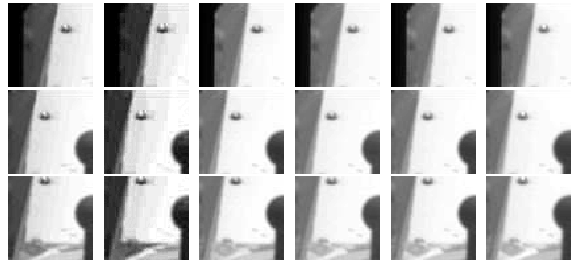
\includegraphics[width=\linewidth]{Raw images gray.png}
  \caption{Sample tiles from the original dataset: typical (non-anomalous).}
  \label{fig:dataset-samples}
\end{figure}

\subsection{Global CP (PARAFAC) Decomposition}

I individually applied a global CANDECOMP/PARAFAC (CP) decomposition to the training, validation and tests datasets. Each dataset is
stacked as a fourth-order tensor \(\mathcal{X}\in\mathbb{R}^{N\times I\times J\times K}\). The model approximates \(\mathcal{X}\) as
\[
\mathcal{X} \;\approx\; \sum_{r=1}^{R}\lambda_r \, h_r \!\circ a_r \!\circ b_r \!\circ c_r,
\]
yielding factor matrices \(H\in\mathbb{R}^{N\times R}\),
\(A\in\mathbb{R}^{I\times R}\), \(B\in\mathbb{R}^{J\times R}\),
\(C\in\mathbb{R}^{K\times R}\), and non-negative component weights
\(\boldsymbol{\lambda}\in\mathbb{R}^{R}\).
Each index in the sample mode \(N\) corresponds to an image tile \(X\in\mathbb{R}^{I\times J\times K}\).
For the training dataset, \(N=1500\), \(I=J=64\), and \(K=6\); the validation and test datasets each have \(N=200\) with the same \(I=J=64\) and \(K=6\).

Columns of \(A,B,C\) capture shared spatial and spectral patterns,
while each row of \(H\) contains per-tile coefficients.
The compression level (rank \(R\)) is chosen during anomaly detection model training via a grid search driven by the best receiver operating characteristic - area under curve (ROC-AUC) achieved with the validation dataset,
with the practical constraint \(R\le \min(IJ,JK,IK)=385\)
(see, e.g., \citep{KoldaBader2009,Bro1997}).

\noindent To obtain scale-consistent per-sample coefficients,
the CP component weights \(\boldsymbol{\lambda}\) are incorporated into the sample-mode factor \(H\).
\[
\tilde H \;=\; H\,\mathrm{diag}(\boldsymbol{\lambda}),
\]
which ensures that each row of \(\tilde H\) reflects the absolute contribution of each component
across samples. Model-specific training and validation
procedures are described in the sections below.

\noindent For validation and test datasets, an additional step is taken to allow comparability with the training dataset. Each image tile \(X\in\mathbb{R}^{I\times J\times K}\)
is embedded into the CP coordinate space defined by the training-fitted factors \((A,B,C)\).
This is done by first computing the componentwise overlaps
\[
g_r \;=\; \big\langle X,\; a_r \circ b_r \circ c_r \big\rangle,
\qquad r=1,\dots,R,
\]
and forming the Hadamard Gram matrix
\[
G \;=\; (A^\top A)\,\ast\,(B^\top B)\,\ast\,(C^\top C),
\]
where \(\circ\) denotes the outer product and \(\ast\) the elementwise (Hadamard) product.
The CP coefficients are then obtained via the least-squares normal equations
\[
Z \;=\; G^{-1} g \;\in\; \mathbb{R}^{\,N \times R}.
\]
following the standard projection approach
\citep{Kiers2000,SorensenBro2009}.

\begin{figure}
  \centering
  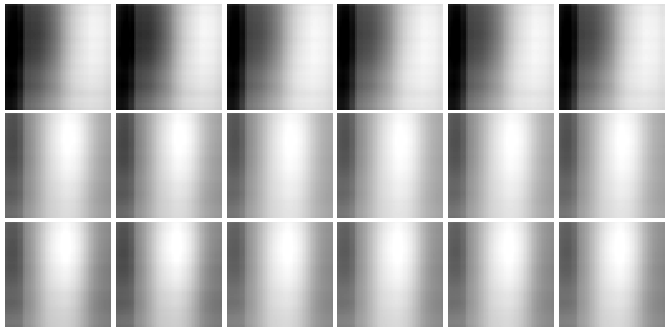
\includegraphics[width=\linewidth]{CP rank 5.png}
  \caption{CP reconstructions at ranks $R = 5$.}
  \label{fig:cp-rank-visuals5}
\end{figure}

\begin{figure}
  \centering
  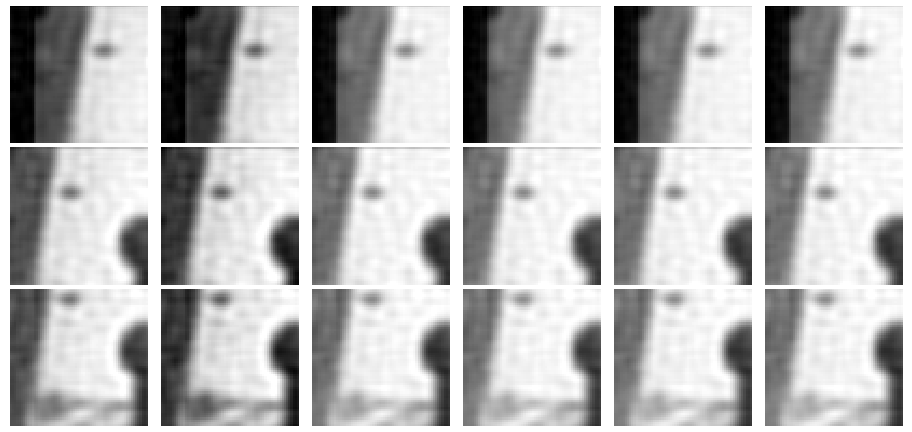
\includegraphics[width=\linewidth]{CP rank 200.png}
  \caption{CP reconstructions at ranks $R = 200$.}
  \label{fig:cp-rank-visuals200}
\end{figure}

\begin{figure}
  \centering
  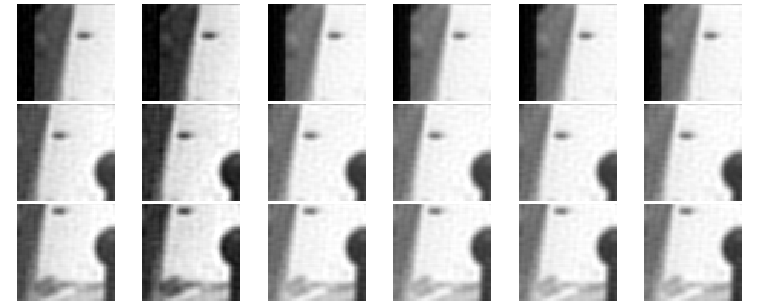
\includegraphics[width=\linewidth]{CP rank 380.png}
  \caption{CP reconstructions at ranks $R = 380$.}
  \label{fig:cp-rank-visuals380}
\end{figure}

\subsection{Tucker Decomposition}

Tucker decomposition is applied to the training, validation and test datasets for each image tile \(X_n \in \mathbb{R}^{64\times 64\times 6}\) given the ranks \((r_1,r_2,r_3)\).
The Tucker model represents each tile via a core tensor and three orthonormal bases (one per mode)
\citep{Tucker1966,KoldaBader2009}:
\[
X_n \;\approx\; \hat X_n \;=\; \mathcal{G}_n \times_{1} U_1 \times_{2} U_2 \times_{3} U_3,
\qquad U_i^\top U_i = I_{r_i},
\]
with dimensions
\[
\mathcal{G}_n \in \mathbb{R}^{r_1\times r_2\times r_3},\quad
U_1 \in \mathbb{R}^{64\times r_1},\quad
U_2 \in \mathbb{R}^{64\times r_2},\quad
U_3 \in \mathbb{R}^{6\times r_3}.
\]
Here, \(\times_n\) denotes the mode-\(n\) tensor-matrix product.

\noindent To perform the decomposition of the image tiles, form a tensor \(\mathcal{X}\) by stacking the image tiles along a sample mode and compute the mode-\(n\) unfoldings \(\mathcal{X}_{(n)}\).
The orthonormal bases are obtained from the left singular vectors of these unfoldings (truncated to rank \(r_n\)) via the
Higher-Order SVD (HOSVD) \citep{DeLathauwer2000a}:
\[
\begin{aligned}
\mathcal{X}_{(1)} &= U_1\,S_1\,V_1^\top \;\;\Rightarrow\;\; U_1 = U_1(:,1{:}r_1),\\[4pt]
\mathcal{X}_{(2)} &= U_2\,S_2\,V_2^\top \;\;\Rightarrow\;\; U_2 = U_2(:,1{:}r_2),\\[4pt]
\mathcal{X}_{(3)} &= U_3\,S_3\,V_3^\top \;\;\Rightarrow\;\; U_3 = U_3(:,1{:}r_3).
\end{aligned}
\]

\noindent With \(U_1,U_2,U_3\) fixed, each tile is projected to its core by three orthogonal projections
\citep{KoldaBader2009}:
\[
\boxed{\;\mathcal{G}_n \;=\; X_n \times_{1} U_1^{\top} \times_{2} U_2^{\top} \times_{3} U_3^{\top}\; }.
\]
This yields a compressed representation that retains dominant multilinear structure while attenuating small, noisy variation
\citep{KoldaBader2009}.

\noindent Each core is vectorized to produce a feature vector
\[
z_n \;=\; \operatorname{vec}(\mathcal{G}_n) \;\in\; \mathbb{R}^{\,r_1 r_2 r_3},
\]
and, for a batch of \(N\) tiles, the feature matrix is
\[
Z \;=\; \begin{bmatrix} z_1^\top \\ \vdots \\ z_N^\top \end{bmatrix}
\;\in\; \mathbb{R}^{\,N \times (r_1 r_2 r_3)}
\]
These vectors \(z_n\) serve as inputs to the downstream anomaly detection models.

Rank is chosen based on the dimension of the tensor being decomposed. In this case, the image dataset has a dimension of 64x64x6. In order to use the full spatial dimensionality of each factor, a search of up to 64 would capture whole spatial variation of the first two factors, while for the third factor, up to rank 6 would capture all its spatial variation.

\begin{figure}
  \centering
  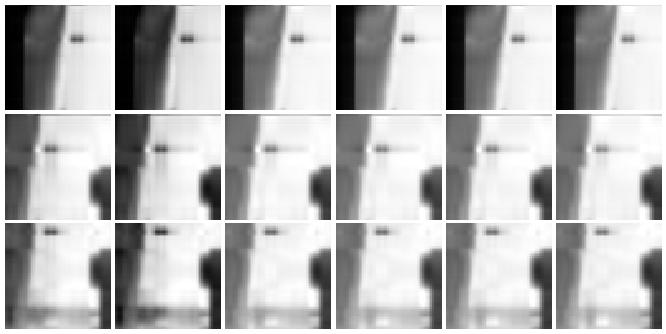
\includegraphics[width=\linewidth]{Tucker rank 5 5 5.png}
  \caption{Tucker reconstructions for (5,5,5).}
  \label{fig:tucker-rank-visuals1}
\end{figure}

\begin{figure}
  \centering
  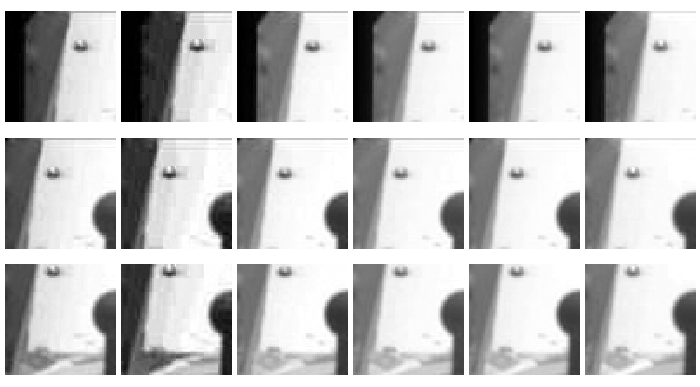
\includegraphics[width=\linewidth]{Tucker rank 32 32 5.png}
  \caption{Tucker reconstructions for (32,32,5).}
  \label{fig:tucker-rank-visuals2}
\end{figure}

\begin{figure}
  \centering
  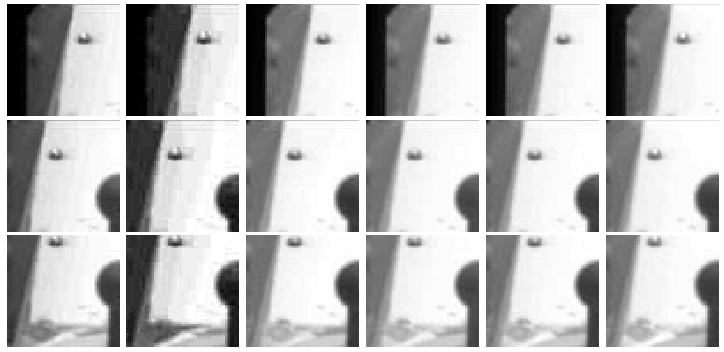
\includegraphics[width=\linewidth]{Tucker rank 64 64 16.png}
  \caption{Tucker reconstructions for (64,64,16).}
  \label{fig:tucker-rank-visuals3}
\end{figure}

\subsection{Standardization}

Given the decomposed training, validation, and test datasets for both CP and Tucker, I standardize the feature vectors and use the standardized features for downstream anomaly detection (one-class SVM, autoencoder, and Isolation Forest) to predict whether an image tile is typical or novel. The per-feature z-score transform is
\[
\tilde{z} \;=\; S(z) \;=\; \frac{z - \mu_{\text{train}}}{\sigma_{\text{train}}} \;\in\; \mathbb{R}^{d},
\]
where \(z\in\mathbb{R}^{d}\) is the feature vector for an image tile, and \(\mu_{\text{train}}\in\mathbb{R}^{d}\), \(\sigma_{\text{train}}\in\mathbb{R}^{d}\) are the mean and standard deviation computed on the \emph{training} features. The same transformation \(S(\cdot)\) is applied to validation and test features (without refitting) to avoid information leakage.

\subsection{One-Class SVM (RBF Kernel)}

Let \(\tilde{Z}_{\text{train}}\in\mathbb{R}^{|T|\times d}\) denote the standardized training feature matrix (rows are tiles; columns are CP/Tucker features). I train an OC-SVM model with an RBF kernel \(K(z,z')=\exp\{-\gamma\lVert z-z'\rVert_2^2\}\) \citep{Scholkopf2001,TaxDuin2004}, where it solves the OC-SVM dual formulation
\[
\max_{\alpha}\; -\tfrac{1}{2} \sum_{i,j=1}^{n} \alpha_i \alpha_j K(z_i, z_j)
\quad \text{s.t.} \quad
0 \leq \alpha_i \leq \tfrac{1}{\nu n}, \qquad
\sum_{i=1}^{n} \alpha_i = 1.
\]
In the above model, \(z_i \in \mathbb{R}^{d}\) denotes a training feature vector (rows of the training matrix \(Z\in\mathbb{R}^{n\times d}\)), and \(\nu\) is a hyperparameter.

\noindent Since validation data is typical-only, I minimize the false-positive rate at the default OC-SVM decision boundary \(f(z)=0\) \citep{Scholkopf2001,TaxDuin2004}. Following common practice in one-class/unsupervised evaluation \citep{Chandola2009,Campos2016,Ruff2021}, I minimize the average indicator of nonnegative validation scores:
\[
\min \; \frac{1}{|V|} \sum_{z \in V} \mathbf{1}\!\left[ s_{\text{val}}(z) \geq 0 \right],
\]
where \(V\) is the validation dataset and \(s_{\text{val}}(z)\) is the OC-SVM validation score for sample \(z\), used for anomaly decisions:
\[
s_{\text{val}}(z) \;=\; \sum_{i=1}^{n} \alpha_i\, K(z_i, z) \;-\; \rho.
\]

\noindent The model is tuned over the parameter grid \[
\gamma \in \left\{ \tfrac{t}{d} : t \in \{0.1, 0.3, 1, 3, 10\} \right\}
\;\cup\; \{\text{scale}, \text{auto}\}, \qquad
\nu \in \{0.01, 0.02, 0.05, 0.10, 0.20\},
\]
and evaluated using the validation scores. The test dataset is then used to compute ROC–AUC, and I report the maximum accuracy achievable under the optimal hyperparameters and decomposition rank.


\subsection{Autoencoders}

\noindent Let \(\tilde{Z}_{\text{train}}\in\mathbb{R}^{|T|\times d}\) denote the standardized training feature matrix (rows are tiles; columns are CP/Tucker features). I train a four-layer, fully connected autoencoder with hidden layer size \(H\in\{128,256,384\}\) and bottleneck size \(B\in\{16,32,64\}\): the encoder maps the feature dimension \(\mathbb{R}^{d}\!\to\!\mathbb{R}^{H}\!\to\!\mathbb{R}^{B}\) and the decoder mirrors this back to \(\mathbb{R}^{H}\!\to\!\mathbb{R}^{d}\) \citep{Hinton2006,Goodfellow2016}.

\noindent Encoder is represented as follows:
\[
h_{\text{enc}} = E_{\theta}(\tilde{z}) \in \mathbb{R}^{B}
\]

\noindent Decoder is represented as follows:
\[
\hat{z} = D_{\theta}(h_{\text{enc}}) \in \mathbb{R}^{d}
\]

\noindent Model parameters \(\theta\) are learned by minimizing mean squared reconstruction error on \(\tilde{Z}_{\text{train}}\), a standard objective for autoencoders \citep{Hinton2006,Goodfellow2016}
\[
\theta^{\star}
\;=\;
\arg\min_{\theta}\;
\frac{1}{|T|}\sum_{\tilde{z}\in Z_{\text{train}}}
\frac{1}{d}\,\big\lVert \tilde{z} - f_{\theta}(\tilde{z}) \big\rVert_{2}^{2},
\]
\noindent The anomaly score for a sample \(\tilde{z}\) is its normalized reconstruction error.
\[
s(\tilde{z})
\;=\;
\frac{1}{d}\,\big\lVert \tilde{z} - f_{\theta}(\tilde{z}) \big\rVert_{2}^{2},
\]
\noindent Larger values indicate greater deviation from normal reconstructions \citep{Sakurada2014,ZhouPaffenroth2017}. Since the validation set contains only typical samples, the operating threshold is set by a high validation quantile,
\[
\tau_{\text{val}} \;=\; \operatorname{P95}\!\big( \{\, s(\tilde{z}) : \tilde{z}\in Z_{\text{val}} \,\} \big),
\]
\noindent and predictions follow
\[
\hat{y}(x) \;=\; \mathbf{1}\!\left[\, s(x) \;\ge\; \tau_{\text{val}} \,\right],
\]
\noindent a common calibration strategy for one-class/unsupervised anomaly detection \citep{Chandola2009,Campos2016,Ruff2021}.


\subsection{Isolation Forest}

Isolation Forest builds an ensemble of binary trees on subsamples of the training feature vectors and exploits the fact that anomalies are few and different: they are isolated by random splits in fewer steps than typical points \citep{Liu2008,Liu2012}. Each tree is grown by recursively selecting a feature and a split value uniformly at random and partitioning the node until a single point remains or a depth limit is reached \citep{Liu2008}.

\noindent We explore the following hyperparameter grid:
\[
T \in \{50,100,200\},\quad
p_{\text{sub}} \in \{0.5,0.75,1.0\},\quad
m_f \in \{0.5,0.75,1.0\},\quad
\text{contamination} \in \{0.05,0.10,0.20\},
\]
where \(T\) is the number of trees, \(p_{\text{sub}}\) is the subsample fraction per tree, \(m_f\) is the fraction of features considered per split, and the contamination parameter specifies an assumed anomaly fraction for the model’s default decision threshold (relevant only when using the built-in \texttt{predict}) \citep{Liu2012}. Let \(n_{\text{sub}}=\lfloor p_{\text{sub}}\cdot |T| \rfloor\) denote the resulting subsample size per tree.

\noindent For a feature vector \(z\), the anomaly score is
\[
s(z) \;=\; 2^{-\bar{h}(z)/c(n_{\text{sub}})}, 
\qquad
\bar{h}(z) \;=\; \frac{1}{T}\sum_{t=1}^{T} h_t(z),
\]
where \(h_t(z)\) is the path length of \(z\) in tree \(t\), and \(c(n_{\text{sub}})\) normalizes scores across subsample sizes \citep{Liu2008}:
\[
c(n_{\text{sub}}) \;=\; 2\,H_{\,n_{\text{sub}}-1} \;-\; \frac{2(n_{\text{sub}}-1)}{n_{\text{sub}}},
\qquad
H_m \;=\; \sum_{k=1}^{m}\frac{1}{k} \;\approx\; \ln(m)+\gamma,
\]
with \(H_m\) the \(m\)-th harmonic number and \(\gamma\) the Euler–Mascheroni constant.

\noindent Because the validation set contains only typical samples, we calibrate the operating threshold by a high validation quantile \citep{Chandola2009,Campos2016,Ruff2021}:
\[
\tau_{\text{val}} \;=\; \operatorname{P95}\!\big(\{\, s(z_v) : z_v \in V \,\}\big),
\qquad
\hat{y}(z) \;=\; \mathbf{1}\!\left[s(z)\ge \tau_{\text{val}}\right],
\]
so that approximately \(5\%\) of validation points are flagged as anomalous. The model with the best validation performance under this calibration is then applied to the test set to report ROC–AUC and accuracy.


\section{Experiments}
\label{sec:experiments}

\subsection{Overview}
In Section~3.1, I define the dataset partitioning strategy; Section~3.2 defines the CP decomposition on the datasets; Section~3.3 defines the Tucker decomposition; and Section~3.4 defines standardization of the decomposed datasets. The following sections describe the model training and tests performed using the common decomposed training, validation, and test datasets. I consolidate the discussions for models using CP and Tucker decompositions since they share the same anomaly–detection models and differ only in the input decomposition technique. Two dataset configurations are evaluated: (i) an \textit{in-order} split using the first 1,500 training tiles, and (ii) a \textit{randomized} selection drawn from the full dataset to assess robustness to sampling diversity.

\subsection{CP/Tucker Rank Search}
For CP decomposition, I sweep the rank \(R \in \{5,10,15,\dots,380\}\).
For Tucker decomposition, I sweep \((R_1,R_2,R_3)\) where
\(R_1,R_2 \in \{5,16,32,64\}\) and \(R_3 \in \{5,16\}\).
Please see Sections~3.2 and~3.3 for the rationale behind these rank choices and for details of how each decomposition is applied to the training, validation, and test sets.

The optimal rank for each model is selected based on the validation set using the criteria described in Section~3.5 (for OC-SVM) and Section~3.6 (for autoencoders).  
Tables~\ref{tab:best-ranks-inorder} and~\ref{tab:best-ranks-random} summarize the best-performing ranks identified from the in-order and randomized dataset experiments, respectively.

\begin{table}
\centering
\caption{Best ranks determined from in-order split experiments.}
\label{tab:best-ranks-inorder}
\begin{tabular}{lcc}
\hline
\textbf{Model} & \textbf{Decomposition Type} & \textbf{Best Rank(s)} \\
\hline
OC-SVM         & CP     & 120 \\
OC-SVM         & Tucker & (32, 32, 16) \\
Autoencoder     & CP     & 35 \\
Autoencoder     & Tucker & (64, 32, 5) \\
Isolation Forest & CP     & 365 \\
Isolation Forest & Tucker & (64, 16, 5) \\
\hline
\end{tabular}
\end{table}

\begin{table}
\centering
\caption{Best ranks determined from randomized split experiments.}
\label{tab:best-ranks-random}
\begin{tabular}{lcc}
\hline
\textbf{Model} & \textbf{Decomposition Type} & \textbf{Best Rank(s)} \\
\hline
OC--SVM         & CP     & 15 \\
OC--SVM         & Tucker & (64, 16, 5) \\
Autoencoder     & CP     & 230 \\
Autoencoder     & Tucker & (64, 64, 5) \\
Isolation Forest & CP     & 315 \\
Isolation Forest & Tucker & (64, 5, 5) \\
\hline
\end{tabular}
\end{table}

Separate rank searches were conducted for both dataset configurations.


\subsection{CP/Tucker Decomposition + OC-SVM}
Given the decomposed training, validation, and test datasets, I fit an OC\mbox{--}SVM on the decomposed training data for each decomposition rank and perform a grid search over:
\[
\gamma \in \Bigl\{ \tfrac{t}{d} : t \in \{0.1,\,0.3,\,1,\,3,\,10\} \Bigr\} \cup \{\texttt{scale}, \texttt{auto}\},
\qquad
\nu \in \{0.01,\,0.02,\,0.05,\,0.10,\,0.20\},
\]
where \(d\) is the feature dimension.

\paragraph{Model selection on typical-only validation.}
Let \(s_{\text{val}}\) be the anomaly scores on the validation set (higher means more anomalous). Because validation contains only typical samples, I select the model by lexicographic minimization:
\[
\min \bigl(\mathrm{FP}@0,\; \mathrm{P95}(s_{\text{val}}),\; \mathrm{mean}(s_{\text{val}})\bigr),
\]
where \(\mathrm{FP}@0\) is the false-positive rate at threshold \(0\), \(\mathrm{P95}\) is the 95th percentile, and \(\mathrm{mean}\) is the sample mean. Intuitively, I first minimize false alarms; ties are broken by preferring tighter and lower score distributions on normals. The rank and OC\mbox{--}SVM hyperparameters achieving this criterion are then evaluated on the test set, and ROC--AUC is reported. Separate rank searches are performed for the in-order and randomized dataset configurations to compare stability and generalization.

\subsection{CP/Tucker Decomposition + Autoencoder}
Given the decomposed training, validation, and test datasets, I fit the autoencoder (defined in Section~3.6) on the training data and validate on the validation set. The optimal rank is chosen as the one yielding the smallest reconstruction error on validation. The chosen rank is then evaluated on the test dataset, and ROC--AUC is reported. This procedure is repeated for both the in-order and randomized splits.

\subsection{CP/Tucker Decomposition + Isolation Forest}
Given the decomposed training, validation, and test datasets, I fit an Isolation Forest on the training data for each decomposition rank and perform a grid search to minimize the validation anomaly score. The selected model is then evaluated on the test dataset. The grid is:
\[
T \in \{50,100,200\},\quad
p_{\text{sub}} \in \{0.5,0.75,1.0\},\quad
m_f \in \{0.5,0.75,1.0\},\quad
\text{contamination} \in \{0.05,0.10,0.20\}.
\]
As with the other models, evaluations are performed separately on both dataset configurations.

\subsection{Raw-Pixel Anomaly Detection}
To establish baselines, I also run OC\mbox{--}SVM, the autoencoder, and Isolation Forest directly on raw-pixel datasets (without decomposition). These baselines allow comparison to determine whether decomposition-based features provide an advantage for anomaly detection under both in-order and randomized splits.

\subsection{Reproducibility and Compute}
I make the code available to aid reproducibility. Experiments were run on the following hardware:
\begin{itemize}
  \item Microsoft Azure D16 Standard: 12 CPU, 64\,GB RAM, no GPU.
  \item Dell workstation: 12 CPU, 64\,GB RAM, NVIDIA RTX A3000 GPU.
\end{itemize}


\section{Results}
\label{sec:results}

This study evaluated three standard anomaly detection models-OC-SVM, autoencoders (AE), and Isolation Forest (IF). These models were trained both on raw pixel data and on data decomposed using tensor methods. Performance was assessed under two setups as described in Section 3.1: (i) an in-order split using the first 1500 datapoints for training and validation, and (ii) a randomized selection from the full dataset.  

\subsection{Baseline Models}
OC-SVM, autoencoders, and isolation forest models were trained and validated on the reduced dataset defined in Section 3.1. These baseline models, used without tensor decomposition, provide a reference for the composite models discussed later. Tables \ref{tab:baseline_result_part1} and \ref{tab:baseline_result_part2} present ROC-AUC values for the baseline models evaluated on the test set and the anomaly categories.

\begin{table}
\centering
\begin{tabular}{lcccccc}
\hline
\textbf{Model} & \textbf{Test set} & \textbf{bedrock} & \textbf{broken-rock} & \textbf{drill-hole} & \textbf{drt} & \textbf{dump-pile} \\
\hline
OC-SVM & 0.5625 & 0.2918 & 0.4070 & 0.4680 & 0.6420 & 0.4940 \\
AE     & 0.5418 & 0.5372 & 0.5971 & 0.4604 & 0.4724 & 0.4512 \\
IF     & 0.6094 & 0.8512 & 0.8743 & 0.3301 & 0.2454 & 0.3163 \\
\hline
\end{tabular}
\caption{Performance of baseline models across categories up to \textit{dump-pile}.}
\label{tab:baseline_result_part1}
\end{table}

\begin{table}
\centering
\begin{tabular}{lccccc}
\hline
\textbf{Model} & \textbf{float} & \textbf{meteorite} & \textbf{scuff} & \textbf{veins} \\
\hline
OC-SVM & 0.2990 & 0.4820 & 0.1320 & 0.7630 \\
AE     & 0.6821 & 0.4689 & 0.5486 & 0.6911 \\
IF     & 0.8889 & 0.6894 & 0.6042 & 0.9300 \\
\hline
\end{tabular}
\caption{Performance of baseline models across categories from \textit{float} to \textit{veins}.}
\label{tab:baseline_result_part2}
\end{table}

\subsection{Rank Selection Summary}
Tables~\ref{tab:best_ranks_inorder} and~\ref{tab:best_ranks_random} summarize the optimal ranks selected by validation for each decomposition–detector combination under the in-order and randomized configurations. All results reported below use these selected ranks.

\begin{table}
\centering
\begin{tabular}{lc}
\hline
\textbf{Model} & \textbf{Best Rank(s)} \\
\hline
CP + OC-SVM    & 120 \\
Tucker + OC-SVM& (32, 32, 16) \\
CP + AE        & 35 \\
Tucker + AE    & (64, 32, 5) \\
CP + IF        & 365 \\
Tucker + IF    & (64, 16, 5) \\
\hline
\end{tabular}
\caption{Optimal ranks (in-order split).}
\label{tab:best_ranks_inorder}
\end{table}

\begin{table}
\centering
\begin{tabular}{lc}
\hline
\textbf{Model} & \textbf{Best Rank(s)} \\
\hline
CP + OC-SVM    & 15 \\
Tucker + OC-SVM& (64, 16, 5) \\
CP + AE        & 230 \\
Tucker + AE    & (64, 64, 5) \\
CP + IF        & 315 \\
Tucker + IF    & (64, 5, 5) \\
\hline
\end{tabular}
\caption{Optimal ranks (randomized split).}
\label{tab:best_ranks_random}
\end{table}

\subsection{CP Decomposition}
The CP results reported below use the optimal ranks in Tables~\ref{tab:best_ranks_inorder} and~\ref{tab:best_ranks_random}.  

For the in-order split (Tables \ref{tab:inOrder_cp_results_part1} and \ref{tab:inOrder_cp_results_part2}), CP + OC-SVM improved ROC-AUC from 0.56 to 0.71 on the test set, with substantial gains in categories such as bedrock, broken-rock, float, meteorite, scuff, and veins. CP + AE showed more modest gains on the test set (0.58 vs.\ 0.54 baseline), with improvements across several categories but declines for bedrock, float, and veins. CP + IF improved slightly on the test set (0.64 vs.\ 0.60 baseline), though performance declined for bedrock, broken-rock, float, meteorite, and veins categories.  

For the randomized selection (Tables \ref{tab:random_cp_results_part1} and \ref{tab:random_cp_results_part2}), CP decomposition generally underperformed compared to the raw-pixel baselines. CP + OC-SVM dropped from 0.56 to 0.49, CP + AE from 0.64 to 0.54, and CP + IF from 0.65 to 0.50, with only minor gains observed in isolated categories such as broken-rock.  

% --- CP Tables ---
\begin{table}
\centering
\begin{tabular}{lcccccc}
\hline
\textbf{Model} & \textbf{Test set} & \textbf{bedrock} & \textbf{broken-rock} & \textbf{drill-hole} & \textbf{drt} & \textbf{dump-pile} \\
\hline
CP + OC-SVM & 0.7095 & 0.6860 & 0.8002 & 0.5625 & 0.3681 & 0.4768 \\
CP + AE     & 0.5778 & 0.5321 & 0.6055 & 0.6597 & 0.6389 & 0.5662 \\
CP + IF     & 0.6487 & 0.7567 & 0.9256 & 0.1597 & 0.1944 & 0.3311 \\
\hline
\end{tabular}
\caption{Performance of in-order CP-based models across categories up to \textit{dump-pile}.}
\label{tab:inOrder_cp_results_part1}
\end{table}

\begin{table}
\centering
\begin{tabular}{lccccc}
\hline
\textbf{Model} & \textbf{float} & \textbf{meteorite} & \textbf{scuff} & \textbf{veins} \\
\hline
CP + OC-SVM & 0.6697 & 0.6817 & 0.4722 & 0.9156 \\
CP + AE     & 0.4969 & 0.7076 & 0.6597 & 0.6311 \\
CP + IF     & 0.9414 & 0.7803 & 0.4097 & 0.9411 \\
\hline
\end{tabular}
\caption{Performance of in-order CP-based models across categories from \textit{float} to \textit{veins}.}
\label{tab:inOrder_cp_results_part2}
\end{table}

\begin{table}
\centering
\begin{tabular}{lcccccc}
\hline
\textbf{Model} & \textbf{Test set} & \textbf{bedrock} & \textbf{broken-rock} & \textbf{drill-hole} & \textbf{drt} & \textbf{dump-pile} \\
\hline
CP + OC-SVM & 0.4914 & 0.4136 & 0.4951 & 0.5023 & 0.5569 & 0.4762 \\
CP + AE     & 0.5405 & 0.6514 & 0.7751 & 0.4711 & 0.3114 & 0.3495 \\
CP + IF     & 0.5048 & 0.6878 & 0.7935 & 0.4029 & 0.3033 & 0.3216 \\
\hline
\end{tabular}
\caption{Performance of randomized CP-based models across categories up to \textit{dump-pile}.}
\label{tab:random_cp_results_part1}
\end{table}

\begin{table}
\centering
\begin{tabular}{lccccc}
\hline
\textbf{Model} & \textbf{float} & \textbf{meteorite} & \textbf{scuff} & \textbf{veins} \\
\hline
CP + OC-SVM & 0.4356 & 0.5218 & 0.5042 & 0.5500 \\
CP + AE     & 0.7292 & 0.6393 & 0.4700 & 0.8088 \\
CP + IF     & 0.7606 & 0.6235 & 0.4458 & 0.8233 \\
\hline
\end{tabular}
\caption{Performance of randomized CP-based models across categories from \textit{float} to \textit{veins}.}
\label{tab:random_cp_results_part2}
\end{table}

\subsection{Tucker Decomposition}
The Tucker results reported below use the optimal ranks in Tables~\ref{tab:best_ranks_inorder} and~\ref{tab:best_ranks_random}. Tucker decomposition produced modest improvements under the in-order split but outperformed CP under randomized selection.  

For the in-order split (Tables \ref{tab:results_inOrder_tucker_part1} and \ref{tab:results_inOrder_tucker_part2}), Tucker + OC-SVM showed a small improvement from 0.54 to 0.57 on the test set, with gains in bedrock, broken-rock, float, meteorite, and scuff. Tucker + AE improved from 0.54 to 0.59, with gains across most categories except drt. Tucker + IF slightly declined from 0.61 to 0.60 on the test set, with performance losses in bedrock, broken-rock, float, meteorite, and veins.  

For the randomized selection (Tables \ref{tab:results_random_tucker_part1} and \ref{tab:results_random_tucker_part2}), Tucker + OC-SVM improved from 0.56 to 0.64, with gains in bedrock, broken-rock, float, meteorite, scuff, and veins. Tucker + AE increased from 0.64 to 0.66 on the test set, though drill-hole, drt, dump-pile, and meteorite declined. Tucker + IF dropped sharply from 0.65 to 0.49, with performance losses across most categories.  

% --- Tucker Tables ---
\begin{table}
\centering
\begin{tabular}{lcccccc}
\hline
\textbf{Model} & \textbf{Test set} & \textbf{bedrock} & \textbf{broken-rock} & \textbf{drill-hole} & \textbf{drt} & \textbf{dump-pile} \\
\hline
Tucker + OC-SVM & 0.5710 & 0.7025 & 0.8131 & 0.3889 & 0.3264 & 0.3842 \\
Tucker + AE     & 0.5900 & 0.6979 & 0.7898 & 0.4653 & 0.4514 & 0.4589 \\
Tucker + IF     & 0.6028 & 0.7968 & 0.7569 & 0.5556 & 0.5000 & 0.4678 \\
\hline
\end{tabular}
\caption{Performance of Tucker-based models across categories up to \textit{dump-pile}.}
\label{tab:results_inOrder_tucker_part1}
\end{table}

\begin{table}
\centering
\begin{tabular}{lcccc}
\hline
\textbf{Model} & \textbf{float} & \textbf{meteorite} & \textbf{scuff} & \textbf{veins} \\
\hline
Tucker + OC-SVM & 0.7346 & 0.5363 & 0.6250 & 0.7567 \\
Tucker + AE     & 0.7160 & 0.5052 & 0.6597 & 0.7956 \\
Tucker + IF     & 0.7469 & 0.6367 & 0.7083 & 0.7689 \\
\hline
\end{tabular}
\caption{Performance of Tucker-based models across categories from \textit{float} to \textit{veins}.}
\label{tab:results_inOrder_tucker_part2}
\end{table}

\begin{table}
\centering
\begin{tabular}{lcccccc}
\hline
\textbf{Model} & \textbf{Test set} & \textbf{bedrock} & \textbf{broken-rock} & \textbf{drill-hole} & \textbf{drt} & \textbf{dump-pile} \\
\hline
Tucker + OC-SVM & 0.6362 & 0.8705 & 0.8872 & 0.5094 & 0.4193 & 0.5654 \\
Tucker + AE     & 0.6643 & 0.8300 & 0.9055 & 0.5486 & 0.4512 & 0.5762 \\
Tucker + IF     & 0.4925 & 0.5027 & 0.5403 & 0.3977 & 0.4230 & 0.5076 \\
\hline
\end{tabular}
\caption{Performance of Tucker-based models across categories up to \textit{dump-pile}.}
\label{tab:results_random_tucker_part1}
\end{table}

\begin{table}
\centering
\begin{tabular}{lcccc}
\hline
\textbf{Model} & \textbf{float} & \textbf{meteorite} & \textbf{scuff} & \textbf{veins} \\
\hline
Tucker + OC-SVM & 0.7692 & 0.7128 & 0.8938 & 0.8638 \\
Tucker + AE     & 0.7961 & 0.6662 & 0.9100 & 0.9152 \\
Tucker + IF     & 0.5075 & 0.3699 & 0.6850 & 0.6362 \\
\hline
\end{tabular}
\caption{Performance of Tucker-based models across categories from \textit{float} to \textit{veins}.}
\label{tab:results_random_tucker_part2}
\end{table}


\section{Discussion}

The experiments highlight both the potential and the limitations of tensor decompositions as feature extraction strategies for anomaly detection in multispectral imagery. Two evaluation setups were considered: (i) an in-order split using the first 1500 datapoints for training, and (ii) a randomized selection drawn from the full dataset. Together, these provide insight into the comparative strengths of CP and Tucker decompositions.  

\subsection{Improvements Under In-Order Splits}

When trained on the first 1500 datapoints in sequence, CP decomposition produced substantial improvements over baseline models. CP + OC-SVM in particular raised overall ROC-AUC from 0.56 (raw OC-SVM) to 0.71, with large category-level gains for bedrock, broken-rock, and veins (up to 0.40 AUC improvement). These results suggest that CP’s global rank structure is highly effective at capturing dominant spatial–spectral patterns when training data is locally coherent, enhancing separability for downstream classifiers such as OC-SVM and Isolation Forest. The optimal ranks identified for these models (\(R=120\) for CP + OC-SVM, \(R=35\) for CP + AE, and \(R=365\) for CP + IF) suggest that moderate to high global ranks were required to achieve maximal separation, emphasizing the capacity of CP to represent locally consistent spatial–spectral structure.  

\subsection{Robustness Under Randomized Sampling}

In contrast, when training samples were drawn at random across the full dataset, CP decomposition underperformed relative to baselines. CP + OC-SVM dropped to 0.49 ROC-AUC, below raw OC-SVM (0.56), with similar degradations for CP + AE and CP + IF. This indicates that CP’s single-rank factorization, while effective on homogeneous subsets, struggles to generalize under heterogeneous sampling.  

Tucker decomposition, however, demonstrated greater stability. Tucker + OC-SVM achieved 0.64 ROC-AUC, surpassing its baseline (0.56), while Tucker + AE also improved slightly (0.66 vs.\ 0.64). Gains were evident across multiple categories, though performance stagnated or declined for drill-hole, drt, and dump-pile. The optimal ranks for Tucker under randomized sampling—particularly \((64,16,5)\) for OC-SVM and \((64,64,5)\) for AE—indicate that higher spatial ranks improved flexibility while keeping compact spectral dimensions, contributing to its stability under heterogeneous conditions. These results highlight Tucker’s ability to flexibly allocate rank across modes, distributing spectral and spatial variability in a way that generalizes more effectively to diverse data. Isolation Forest, while strong as a baseline, showed limited benefit or degradation when paired with decompositions, suggesting it already captures variance structure effectively in raw feature space.  

\subsection{Category-Specific Recommendations}

The category-level analysis suggests that CP and Tucker decompositions offer complementary strengths. For locally coherent data, CP + OC-SVM yielded substantial improvements in anomalies such as bedrock, broken-rock, and veins, where global rank structure captures shared spectral–spatial patterns. For more heterogeneous anomaly types, Tucker decomposition proved more reliable, consistently outperforming baselines for categories including bedrock, broken-rock, float, scuff, and veins under randomized sampling. These findings indicate that decomposition choice can be tailored to the anomaly type of interest rather than applied as a one-size-fits-all strategy. These category-specific differences also align with the rank-search outcomes: CP required larger ranks to capture localized consistency, while Tucker achieved strong performance with compact yet balanced rank configurations.  

\subsection{Trade-Off Between Potential and Stability}

Overall, the two experiments reveal a trade-off between potential gain and robustness. CP decomposition provides striking improvements when training data is locally consistent and representative of test conditions, but its performance deteriorates under randomized sampling. Tucker decomposition delivers more modest improvements in structured splits yet maintains stable or superior performance under heterogeneous conditions. From a practical perspective, this robustness makes Tucker decomposition a stronger candidate for deployment in real-world scenarios where training data must capture diverse and unpredictable distributions.  

\subsection{Considerations}

While the current experiments demonstrate the utility of CP and Tucker decompositions for anomaly detection in multispectral imagery, several directions remain open. First, training was performed on relatively limited subsets (e.g., 1500 datapoints). Expanding the training pool could enable both CP and Tucker models to learn more representative latent factors, mitigating CP’s sensitivity to heterogeneity and strengthening generalization.  

Second, the number of anomaly test samples was limited. Incorporating additional labeled anomalies, either through annotation or synthetic augmentation, would allow more robust estimation of model sensitivity across categories and clarify whether CP’s advantages on structured anomalies and Tucker’s stability under heterogeneous data persist at scale.  

Finally, tensor decomposition methods should be applied to additional datasets. While this study focused on multispectral rover imagery, CP and Tucker factorizations are general techniques that extend to other domains such as medical imaging (MRI, CT) and industrial inspection. Benchmarking across diverse datasets will help determine whether the category-specific advantages observed here generalize and be broadly applicable.  


\section{Conclusion}
\label{sec:conclusion}

This work evaluated the use of tensor decomposition methods, specifically CP and Tucker factorizations, as feature extraction strategies for anomaly detection in multispectral imagery. By comparing models trained on raw pixel data with those trained on decomposed representations, two consistent findings emerged.    

First, CP decomposition demonstrated strong potential under locally coherent training conditions. In in-order splits, CP + OC-SVM in particular achieved substantial improvements, raising ROC-AUC by as much as 40\% in certain anomaly categories. These results highlight the power of global CP structure in capturing dominant spectral–spatial patterns when training and test distributions are aligned. The optimal ranks identified for the in-order setup (\(R=120\) for CP + OC-SVM and \(R=365\) for CP + IF) further underscore the role of high-rank global structure in modeling consistent data.  

Second, Tucker decomposition exhibited greater robustness under heterogeneous conditions. In randomized sampling, Tucker-based models consistently outperformed both baselines and CP-based pipelines, achieving the highest overall test set ROC-AUC and providing reliable gains across multiple categories. These outcomes suggest that Tucker’s ability to flexibly allocate rank across modes makes it more adaptable to diverse data distributions. Across experiments, the optimal rank search revealed that CP models favored higher ranks (e.g., 120–365), while Tucker models achieved competitive or superior results with lower, mode-specific ranks (e.g., \(32,32,16\) or \(64,16,5\)), underscoring Tucker’s efficiency in representing heterogeneous structure.  

Taken together, the results indicate a trade-off between potential and stability. CP offers the greatest performance gains in structured regimes, while Tucker provides more reliable performance in settings where variability and heterogeneity are high. From an applied perspective, this suggests that the choice of decomposition strategy should depend on the data characteristics and the anomaly categories of interest.  

Future work will involve scaling the training sets, expanding anomaly annotations, and applying these methods to additional domains such as medical imaging or industrial inspection. Such efforts will help determine whether the category-specific strengths observed here generalize across broader contexts.  

Overall, this study shows that tensor decompositions can substantially enhance anomaly detection pipelines, provided their use is tailored to the structure of the data and the deployment setting.


\section*{Acknowledgments}
This work was conducted as part of the author’s practicum project in the Online Master of Science in Analytics (OMSA) program at the Georgia Institute of Technology. The author gratefully acknowledges the Mars multispectral image dataset prepared and analyzed by \citep{Kerner2020}, which provided the datasets for this study. The author also thanks the OMSA faculty and practicum advisors for their guidance during the project.

\section*{Statements and Declarations}

\subsection*{Funding}
Not applicable.

\subsection*{Competing Interests}
The author declares that no competing interests exist.

\subsection*{Ethics approval and consent to participate}
Not applicable.

\subsection*{Consent for publication}
Not applicable.

\subsection*{Data availability}
Data sharing is not applicable to this article as no new datasets were generated or analysed.

\subsection*{Code availability}
Code is available on the following github repository: 

\subsection*{Author contribution}
The author confirms being the sole contributor of this work and has approved it for publication.


\bibliography{refs}
\end{document}
